\documentclass[12pt, a4paper]{article}
\usepackage[utf8]{inputenc}
\usepackage{amsmath}
\usepackage{amsthm}
\usepackage{graphicx}
\usepackage{parskip}
\usepackage{hyperref}
\usepackage{fancyhdr}
\usepackage{lastpage}
\usepackage{color}
\usepackage{caption}
\usepackage{float}
\usepackage{algorithm}
\usepackage{algorithmic}
\usepackage[acronym]{glossaries}
\usepackage[nottoc]{tocbibind}
\usepackage{tikz}
\graphicspath{{./images/}}

\DeclareMathOperator*{\argmax}{arg\,max}
\DeclareMathOperator*{\argmin}{arg\,min}

\renewcommand{\algorithmicrequire}{\textbf{Input}}
\renewcommand{\algorithmicensure}{\textbf{Output}}

\title{%
      Homework 2 \\
      Kd-Trees
}
\author{%
  Juan Pablo Royo Sales\\
  \small{Universitat Politècnica de Catalunya}
}
\date\today

\pagestyle{fancy}
\fancyhf{}
\fancyhead[C]{}
\fancyhead[R]{Juan Pablo Royo Sales - UPC MIRI}
\fancyhead[L]{ADM - Kd-Trees}
\fancyfoot[L,C]{}
\fancyfoot[R]{Page \thepage{} of \pageref{LastPage}}
\setlength{\headheight}{15pt}
\renewcommand{\headrulewidth}{0.4pt}
\renewcommand{\footrulewidth}{0.4pt}

\makeglossaries

\newacronym{kdt}{K-d Tree}{K-Dimensional Binary Search Tree}
\newacronym{bst}{BST}{Binary Search Tree}
\newacronym{nns}{NNS}{Nearest Neighbor Search}
\newacronym{lsh}{LSH}{Locality Sensitivity Hashing}

\begin{document}

\maketitle

\medskip

\section{Introduction}
A \textbf{\acrfull{kdt}} was defined by first time in \cite{bentley} is a Multidimensional Data Structure and a generalization of a \textbf{\acrfull{bst}} but with discriminators by level. In the following sections we are going to describe formally this structure.

\acrshort{kdt} can be \textbf{Standard} which is the definition given by \cite{bentley} or \textbf{Relaxed} which implements a Randomized selection of the discriminators at each level. In this article we are going to describe and focus only in \textbf{Standard} \acrshort{kdt}.

The idea of this article is to show the power of \acrshort{kdt} for running \acrfull{nns} algorithm in order to be tested against \acrfull{lsh} in a posterior work.

\section{Definition}
A \textbf{\acrshort{kdt}} of size $n \geq 0$ contains a Set $n$ $K$-dimensional records, such that each key $x = (x_0, \dots , x_{K-1}) \in D$ where  $D = D_0 \times \dots \times D_{K-1}$, and each $D_j, 0 < j < K$, is a totally ordered domain.

A \textbf{\acrshort{kdt}} $T$ is a \acrshort{bst} such that:

\begin{itemize}
    \item If $n = 0$ then $T$ is empty
    \item Root's $T$ stores a pair $(x,d)$ given that $x$ is the key of one of the $K$-dimensional points and $d$ is the level or discriminant of the node such that $ d = \text{root level } mod K, 0 \leq j < K$
    \item A left $L$ and right $R$ subtree is build recursively with the following form: $ L = \{ x_i | x_i < x_{root} \}$ and $R = \{x_j | x_j > x_{root}\}$.
    \item Each level of the tree use the same discriminator $d$.
\end{itemize}

The following example that was taken from \cite{vtech_page} illustrate the definition given above:

\begin{minipage}[t]{\linewidth}
  \includegraphics[width=\textwidth]{KDTree}
  \captionsetup{type=figure}
  \captionof{figure}{Example of KDTree}
  \label{fig:kdtree_example}
\end{minipage}

As we can see in this example \acrshort{kdt} divides the \textit{space} in \textit{hyperrectangles}. As we can see here point $A$ which is the first inserted use as a discriminator dimension $x$, so in the next level discriminator will be $y$ and after that $x$ again.

\acrshort{kdt} are optimal for doing any kind of range query, as well as exact search, partial matches and of course \acrshort{nns} searches.

\subsection{Characteristics}
In the case of cost analysis on \acrshort{kdt} we should distinguish different kinds of cost:

\begin{itemize}
  \item Construction cost: $\Theta(n\log{n})$ worst case
  \item Storage cost: $\Theta(n)$ worst case
  \item Range Query cost: $\Theta(R + n^{1 - \frac{s}{K} + \Theta(\frac{s}{K})})$ in average, where $R$ is the number of points in the range.
  \item Near Neighbor Search cost: $O(\log{n} + R)$ according to \cite{fried} average case for small answer.
\end{itemize}

We are going to focusing in the Cost analysis of \acrshort{nns} which is the goal of our work for doing predictions and comparing in a future work with \acrshort{lsh}.


\section{Near Neighbor Search Analysisi}

Given a \acrshort{kdt} with $N$ nodes, without doing a rough analysis we can say that on average, at least $O(\log{N})$ visits are necessary, because any \acrshort{nns} algorithm requires traverse to at least one \textbf{leaf} of the tree. It is obvious that there is no need to visit more than $N$ since the algorithm inspect each node at most once.

Since we want to know how well it performed for future empirical analysis comparison against \acrshort{lsh}, we want to know the worst case number of visited nodes and the \textbf{expected} one to see the average case.


\begin{minipage}[t]{\linewidth}
  \begin{center}
    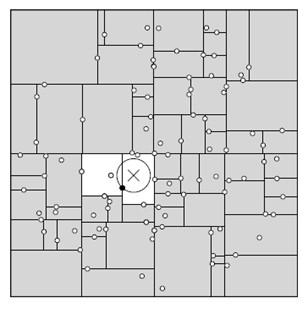
\includegraphics{kdt_1}
  \end{center}
  \captionsetup{type=figure}
  \captionof{figure}{KDTree example construction for analysis}
  \label{fig:kdt_1}
\end{minipage}


\begin{minipage}[t]{\linewidth}
   \begin{center}
    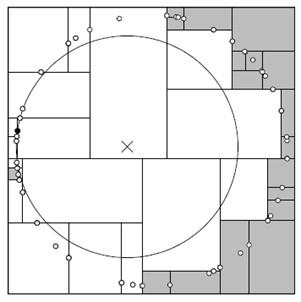
\includegraphics{kdt_2}
  \end{center}
  \captionsetup{type=figure}
  \captionof{figure}{KDTree zoom on worst distribution of points}
  \label{fig:kdt_2}
\end{minipage}

As we can see in the \ref{fig:kdt_1} that was extracted from \cite{moore_phd}, this distribution example shows us that we are going to visit much more less nodes than $N$ because all the grey areas can be discarding while searching.

On the other hand \ref{fig:kdt_2} shows how a bad distribution will lead us to visit almost every node in a worst case scenario.

In the case of the expected number of nodes visited analysis, as we can see on \cite{fried}, this analysis is based on the \textbf{expected} number of \textbf{hyperrectangles} corresponding to a leaf node with high probability of being inspected. That hyperrectangles intersect the hypersphere corresponding with the query point $x$. In the image \ref{fig:kdt_1} it is the hypersphere of the circle marked with $X$. In this example the number of hyperrectangles is 2 because it is easy to see that the circle is intersecting them.

The asymptotic search time analysis in \cite{fried} shows that it is $O(\log{n})$ because the required time to descend from the root to a \textit{terminal bucket}, as it is called in \cite{fried} for leaves nodes, is logarithmic in the number of nodes, which is directly proportional to the size of $N$.

As it is pointed out in the analysis, we need also take into consideration the \textit{backtracking} in the tree since we need to go back to visit nodes that we need still visit because each level of the tree represents a specific dimension. As it is shown in the paper, the amount of backtracking in search is $\overline{l}$, which is the expected number of buckets overlapped by the Search region.

\begin{equation*}
\overline{l} \leq \overline{L} = \{[(m/b)G(k)]^{1/k}\}^k
\end{equation*}

Where $\overline{L}$ represents the average number of buckets overlapped by the search region. As we can see this number does not depend on $N$. Therefore the expected number of search time is proportional to $\log{N}$.


\section{Conclusion}
As we have seen \acrshort{kdt} is a good alternative to explore predictors with reasonable logarithmic average cost on that search.
Although this is what we are going to explore empirically in a next work, we already know that this data structure suffer from what is called the curse of dimensionality and it is what \acrshort{lsh} tries to solve.


\bibliographystyle{alpha}
\bibliography{Homework2_jproyo}

\printglossaries

\end{document}

